% Appendix figures referenced from the Results section. Place inside \appendix.

\begin{figure*}[t]
  \centering
  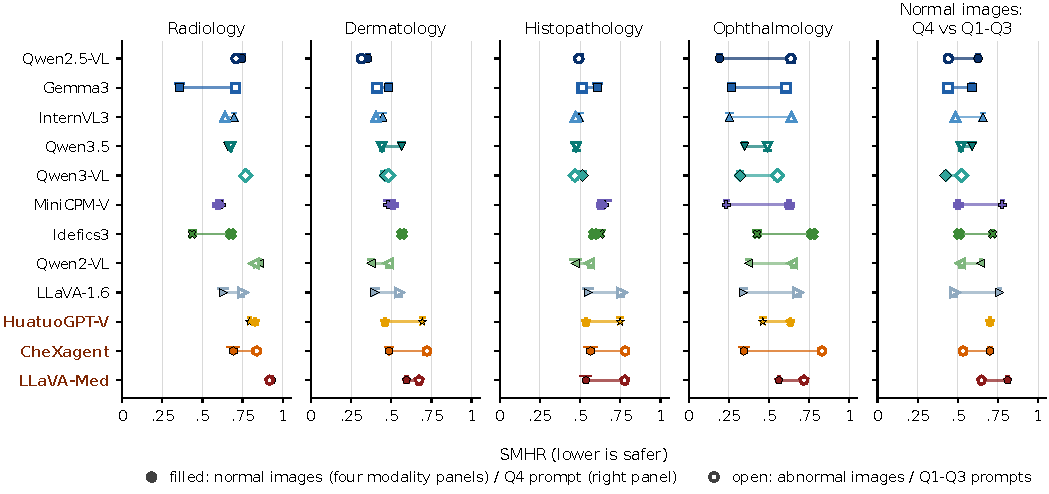
\includegraphics[width=\textwidth]{paper_figures/fig05_normal_image_paradox.pdf}
  \caption{\SMHR{} on normal strata (S1, DS1, HS1, OS1; filled) and abnormal strata (open) for the first three queries by modality (left four panels; 1,250 normal and 2,250 abnormal images), and on normal images for the false-premise query versus the first three queries (right). Bars are 95\% image-level bootstrap intervals (2,000 resamples). The radiology panel is affected by the image issue \rad{}.}
  \label{fig:normal}
\end{figure*}

\begin{figure}[t]
  \centering
  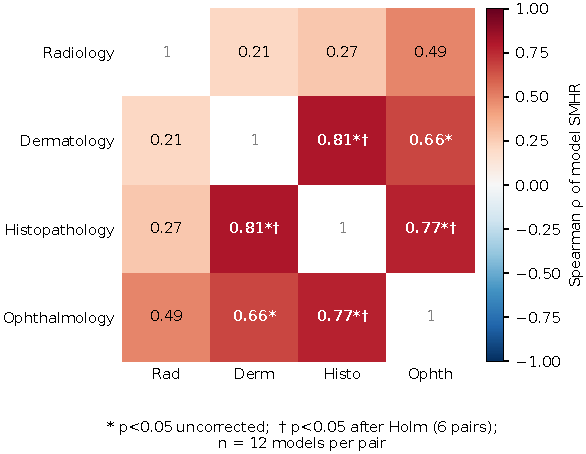
\includegraphics[width=\columnwidth]{paper_figures/fig06_cross_modal_transfer.pdf}
  \caption{Spearman correlation between the rankings of the 12 models by \SMHR{} in each pair of modalities ($n = 12$ models). Marks indicate $p < 0.05$ without ($*$) and with ($\dagger$) Holm correction for six pairs. No confidence intervals are drawn, and with $n = 12$ the weaker correlations are inconclusive. Pairs involving radiology are affected by the image issue \rad{}.}
  \label{fig:transfer}
\end{figure}

\begin{figure*}[t]
  \centering
  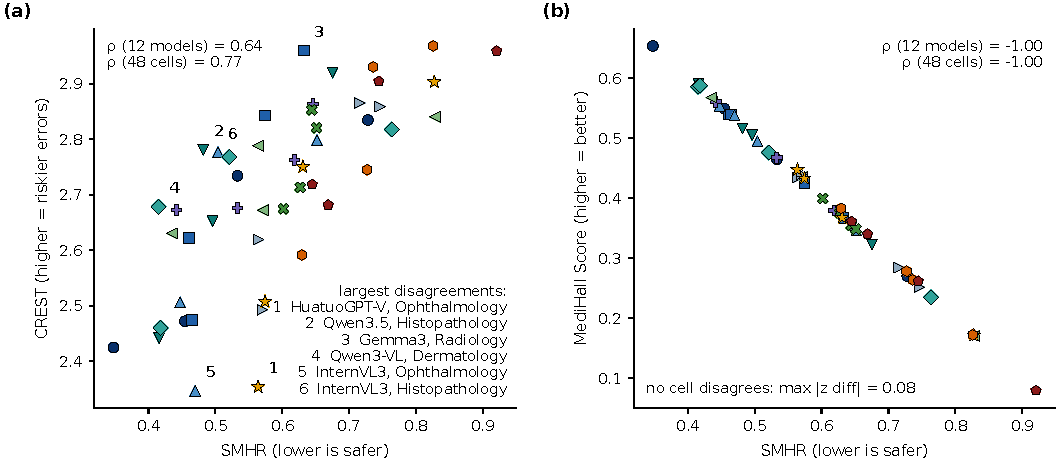
\includegraphics[width=\textwidth]{paper_figures/fig07_metric_concordance.pdf}
  \caption{\SMHR{} against (a) CREST and (b) the MediHall Score for 12 models in 4 modalities (48 cells; one marker per cell, marker shape identifies the model). Spearman $\rho$ is shown for the 12 model-level values and for the 48 cells. Numbered cells are the six largest standardised \SMHR--CREST disagreements. No confidence intervals are shown.}
  \label{fig:concordance}
\end{figure*}

\begin{figure*}[t]
  \centering
  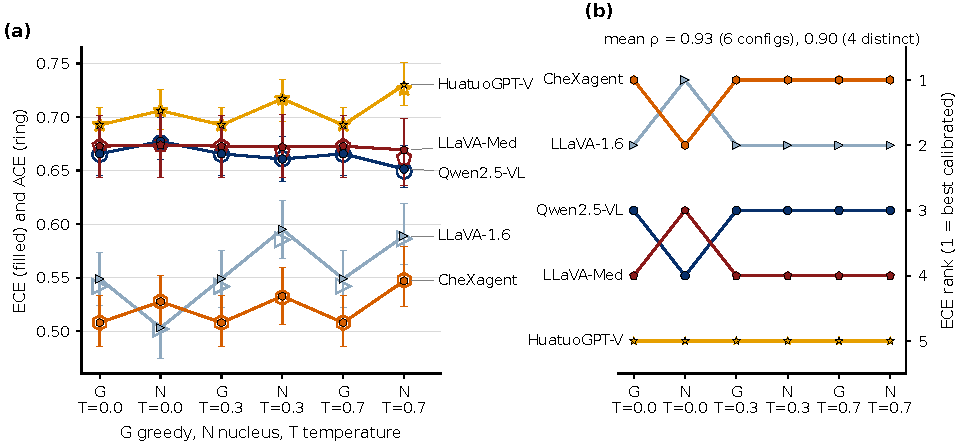
\includegraphics[width=\textwidth]{paper_figures/fig08_calibration.pdf}
  \caption{(a) Expected (ECE) and adaptive (ACE) calibration error of stated confidence for five models under six decoding configurations (strict correctness label; 699 to 1,495 labelled responses per cell from a 500-image subset); bars are 95\% bootstrap intervals on ECE. (b) ECE rank of each model per configuration. Adjacent models whose intervals overlap under greedy decoding (CheXagent and LLaVA-1.6, Qwen2.5-VL and LLaVA-Med, LLaVA-Med and HuatuoGPT-Vision) are not ordered.}
  \label{fig:calibration}
\end{figure*}
% NOTE: the manifest caption for panel (b) reports a mean pairwise rho of 0.93 over six configurations; the audit reports 0.90 over the four distinct settings, because three greedy configurations are identical. Use 0.90.
